\section{目的}
本研究では, 地理的分散環境下における分散グラフ RW 実行エンジンを提案した. 提案手法を既存の分散グラフ RW 実行エンジンである KnightKing \cite{10.1145/3341301.3359634} と比較することで, 地理的分散環境下における本手法の有用性を明らかにする. また, 送信時に RWer をまとめることによる性能向上の評価, そして経路再利用のための再利用エッジデータが貯まるまでの RW 実行数の評価のように本手法の構成要素に関する評価も行った. 

\section{項目}

評価項目は以下の通りである. 
\begin{quote}
    \begin{itemize}
        \item 既存手法との比較
        \begin{itemize}
            \item RTT, パケットロス率を変えた場合の実行時間
            \item Random Walker の経路再利用をした場合の実行時間
            \item グラフ分割精度を変えた場合の実行時間
            \item グラフ分割数 (サーバ台数) を変えた場合の実行時間
            \item Random Walk の終了確率 $\alpha$ を変えた場合の実行時間
        \end{itemize}
        \item 提案手法に関する評価
        \begin{itemize}
            \item Random Walker をまとめて送信したことによる速度向上
            \item 再利用エッジが貯まるまでに実行する Random Walk の回数
        \end{itemize}
    \end{itemize}
\end{quote}

\section{評価環境}

\subsection{データセット}

本評価では実世界グラフと生成グラフの両方を使用して実験を行った. 実世界グラフは LiveJournal のデータセット\cite{snapnets} (頂点数 3,997,962, 辺数 69,362,378) を使用した. 生成グラフに関しては, エッジ生成確率を制御できるアルゴリズムである, Stochastic block model (SBM) \cite{SBM} を使用した. SBM では, partition 数, 各 partition 内の頂点数, partition 内の頂点間のエッジ生成確率, partition 間の頂点間のエッジ生成確率を指定し, グラフを生成することができる. このエッジ生成確率を操作することで, 例えばサーバ間を跨ぐ RW 遷移が多くなるグラフを生成することができる. 生成グラフの頂点数とエッジ生成確率の値に関しては, 実験 \ref{グラフ分割の汚さを変えた場合の実行時間}, \ref{グラフ分割数を変えた場合の実行時間} で説明する. 
実世界グラフは実験 \ref{RTT, パケットロス率を変えた場合の実行時間}, \ref{Random Walker の経路再利用をした場合の実行時間}, \ref{グラフ分割数を変えた場合の実行時間}, \ref{終了確率 alpha を変えた場合の実行時間}, \ref{Random Walker をまとめて送信した場合とそうでない場合の実行時間}, \ref{再利用エッジが貯まるまでに実行する Random Walk 実行数} で使用し, 生成グラフは実験 \ref{グラフ分割の汚さを変えた場合の実行時間}, \ref{グラフ分割数を変えた場合の実行時間} で使用した. 

\subsection{評価環境}

本評価では最大 7 台のサーバを使用して実験を行った. 各サーバは全て同じ性能をしており, 表 \ref{評価環境} に示す. また, 実装は全て C++ で行った. 基準となる評価環境は以下の通りである. 特に指定がない限りはこの設定で実験を行った. 分割数が 5 のハッシュ分割では各サーバの ID を 0 $\sim$ 4 とし, 各頂点をサーバ ID = 頂点 ID \% 5 のサーバに配置する.
\begin{quote}
    \begin{itemize}
        \item サーバ数
        \begin{itemize}
            \item 5 台
        \end{itemize}
        \item グラフ分割
        \begin{itemize}
            \item ハッシュ分割
        \end{itemize}
        \item RTT
        \begin{itemize}
            \item 100 ms
        \end{itemize}
        \item パケットロス率
        \begin{itemize}
            \item 0.03 \%
        \end{itemize}
        \item RW の終了確率 $\alpha$
        \begin{itemize}
            \item 0.15
        \end{itemize}
        \item RWer 経路再利用機能
        \begin{itemize}
            \item なし
        \end{itemize}
    \end{itemize}
\end{quote}

\begin{table}[t]
    \caption{評価環境.}
    \label{評価環境}
    \centering
    \begin{tabular}{c|c}
      \hline
      項目 & 内容   \\
      \hline \hline
      OS  & Ubuntu 20.04 LTS \\
      CPU  & Intel(R) Xeon(R) CPU E5-2643 v2 @ 3.50GHz  \\
      Core & 24 (hyper threading 有効) \\
      RAM  & 32GB \\
      \hline
    \end{tabular}
\end{table}

\subsection{RW 実行について}

本評価における RW 実行のに実行時間について, 開始時間は RWer を生成し始めるタイミングで, 終了時間は全てのサーバで全ての RWer の終了確認が取れたタイミングとしている. 既存手法と異なり提案手法は UDP 通信を使用しているため, パケットロスによる RWer の損失が発生する. 本来提案手法では, RWer の損失の影響が少ない (図 \ref{局所的に RWer が損失したときの PPR 演算の精度} 参照) ことを理由にパケットロスを許容しているが, 全ての RWer の終了を前提としている既存手法との比較のために, 簡易的な再送機能を実装した. 再送スレッドは全体の 95 \% の RW 実行が終了した時点で起動し, 3 秒ごとにまだ終了確認の取れてない RWer を再生成する. 

\section{既存手法との比較}

\subsection{RTT, パケットロス率を変えた場合の実行時間}\label{RTT, パケットロス率を変えた場合の実行時間}

% データセットは実世界グラフ, サーバ数は 5 台で実験を行った. まず, 実験前にグラフを 5 分割し, 各サーバに配置する. ここでの分割方法はハッシュ分割 (ランダム分割) である. 具体的には, 各サーバの ID を 0 $\sim$ 4 とし, 各頂点をサーバ ID = 頂点 ID \% 5 のサーバに配置する. この先特に指定がない場合は, 分割に関してはこのハッシュ分割を採用している. そして RW 実行に関しては, 終了確率 $\alpha$ = 0.15 の RW を各頂点から 10 回ずつ実行する. 実世界グラフの頂点数は 3,997,962 なので実行する RW 数は合計 39,979,620 回となる. 
実世界グラフを用いて, RW を各頂点から 10 回ずつ実行した. 実世界グラフの頂点数は 3,997,962 なので実行する RW 数は合計 39,979,620 回となる.

実験結果を図 \ref{パケットロス率を 0.03 に固定したときの実行時間}, \ref{RTT を 100 ms に固定したときの実行時間} に示す. まず, 図 \ref{パケットロス率を 0.03 に固定したときの実行時間} は, サーバ間のパケットロス率を 0.03 \% に固定し, RTT を 0 $\sim$ 200 ms で変動させて実験を行った結果である. 既存手法では RTT が 0 ms, 50 ms, 100 ms, 150 ms, 200 ms と変化すると実行時間が約 4 秒, 52 秒, 86 秒, 131 秒, 151 秒となり, 大幅に増加していることがわかる. これは既存手法が TCP 通信を使用していることが原因であり, RTT が大きくなるとスループットが小さくなる. 対して提案手法では RTT が 0 ms, 50 ms, 100 ms, 150 ms, 200 ms と変化すると実行時間が約 49 秒, 52 秒, 53 秒, 55 秒, 55 秒となっており, 既存手法と比べてあまり増加しないことがわかる. これは提案手法が UDP 通信を使用しているためであり, RTT が変化してもスループットの変化は小さい. RTT が 0 のときは既存手法が 4 秒, 提案手法が 49 秒と既存手法の方が約 12 倍高速である. これは, 既存手法における RWer の送信では経路情報を送らないため通信量が少ないこと, そして同期処理によって CPU リソースを最大限活用することができていることが要因であると考える. 図 \ref{RTT を 100 ms に固定したときの実行時間} は, サーバ間の RTT を 100 ms に固定し, パケットロス率を 0 $\sim$ 0.1 \% で変動させて実験を行った結果である. こちらも 図 \ref{パケットロス率を 0.03 に固定したときの実行時間} と同様に, パケットロス率の増加とともに実行時間が大きく増加する既存手法に対し, 提案手法では実行時間がほとんど変化していない. これらの結果から, RTT, パケットロス率が無視できるような環境では既存手法のような TCP 通信を使った同期処理による RW 処理, 地理的分散環境のような RTT, パケットロス率が無視できない環境では提案手法のような UDP 通信を使った非同期処理が適していることがわかる. 

\begin{figure}[t]
    \centering
    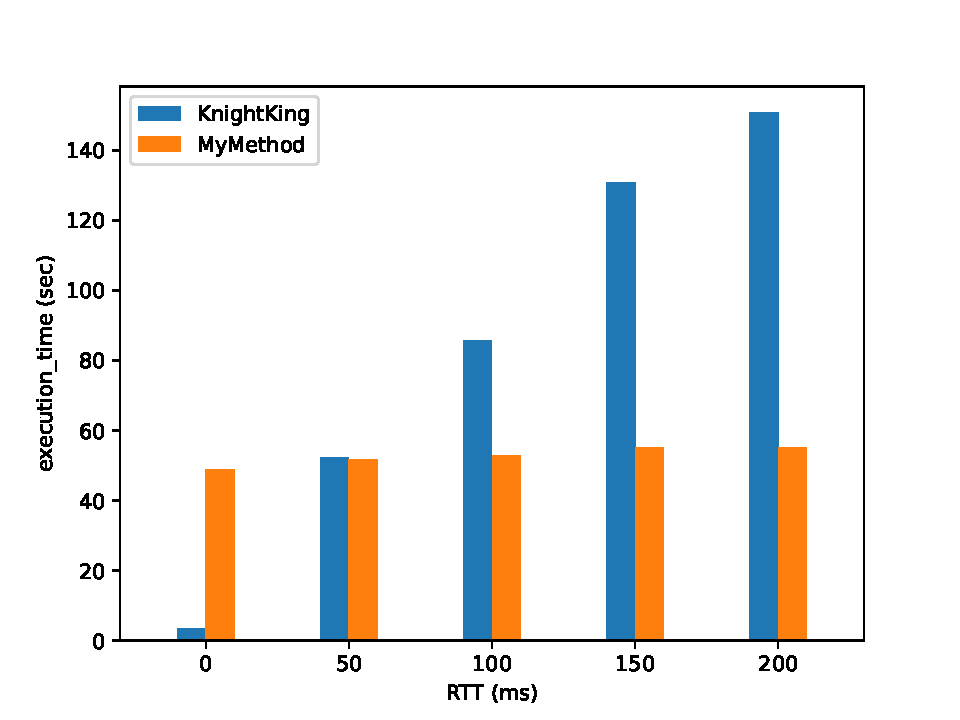
\includegraphics[scale=0.8]{figure/Kn_vs_AR_RTT.pdf}
    \caption{パケットロス率を 0.03 \% に固定したときの実行時間.}
    \label{パケットロス率を 0.03 に固定したときの実行時間}
\end{figure}

\begin{figure}[t]
    \centering
    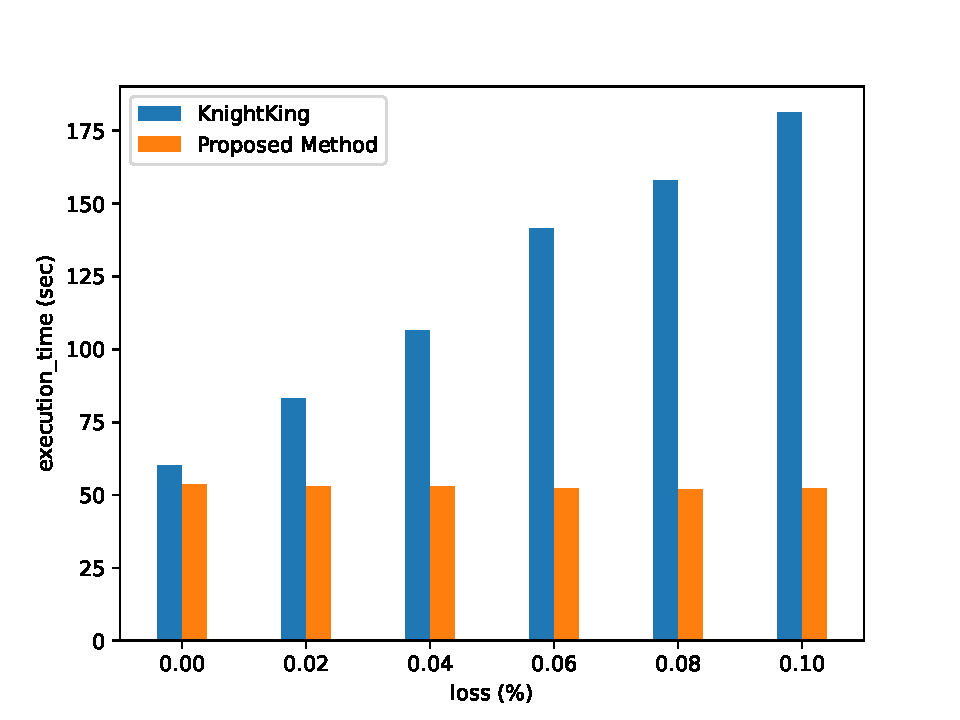
\includegraphics[scale=0.8]{figure/Kn_vs_AR_loss.pdf}
    \caption{RTT を 100 ms に固定したときの実行時間.}
    \label{RTT を 100 ms に固定したときの実行時間}
\end{figure}

\subsection{Random Walker の経路再利用をした場合の実行時間}\label{Random Walker の経路再利用をした場合の実行時間}

実世界グラフを用いて, RW を各頂点から 10 回ずつ実行した. また本実験では, RWer 経路の再利用機能を利用する. 再利用するエッジデータは実験前に調達済みであるとする. 

図 \ref{経路再利用をしたときの実行時間} に経路再利用をしたときの実行時間を示す. 緑の点線は既存手法を, 青い棒は提案手法の経路再利用をしないもの, オレンジ色の棒は提案手法の経路再利用をするものを表す. 横軸における original edges は元々各サーバが保持していたエッジの数であり, reuse edges は再利用エッジの数である. 実世界グラフにおけるエッジの数は全部で 69,362,378 なので, これを 5 分割した約 14,000,000 が original edges の値となる. つまり, original edges + reuse edges = 20,000,000 のとき, reuse edges の値は約 6,000,000 である. 実験結果について, 提案手法の経路再利用をしない場合は既存手法に比べて約 1.6 倍高速であり, 提案手法の経路再利用をする場合はそれぞれ提案手法に比べて約 2.2 倍, 2.9 倍, 3.8 倍, 5.0 倍, 7.2 倍高速だった. 結果から RWer の経路再利用により実行時間を削減できていることがわかる. また, 経路再利用による削減時間を再利用エッジ数で割ることにより, 再利用エッジ 1 本あたりの時間削減量を求めたところ, original edges + reuse edges ($\times$ 10000) = 2000, 3000, 4000, 5000, 6000 でそれぞれ約 0.024, 0.014, 0.012, 0.010, 0.009 になった. この結果から, 再利用エッジが増えれば増えるほど再利用エッジ 1 本あたりの時間削減量が減ることがわかった. 
\\
\\
\\

\begin{figure}[t]
    \centering
    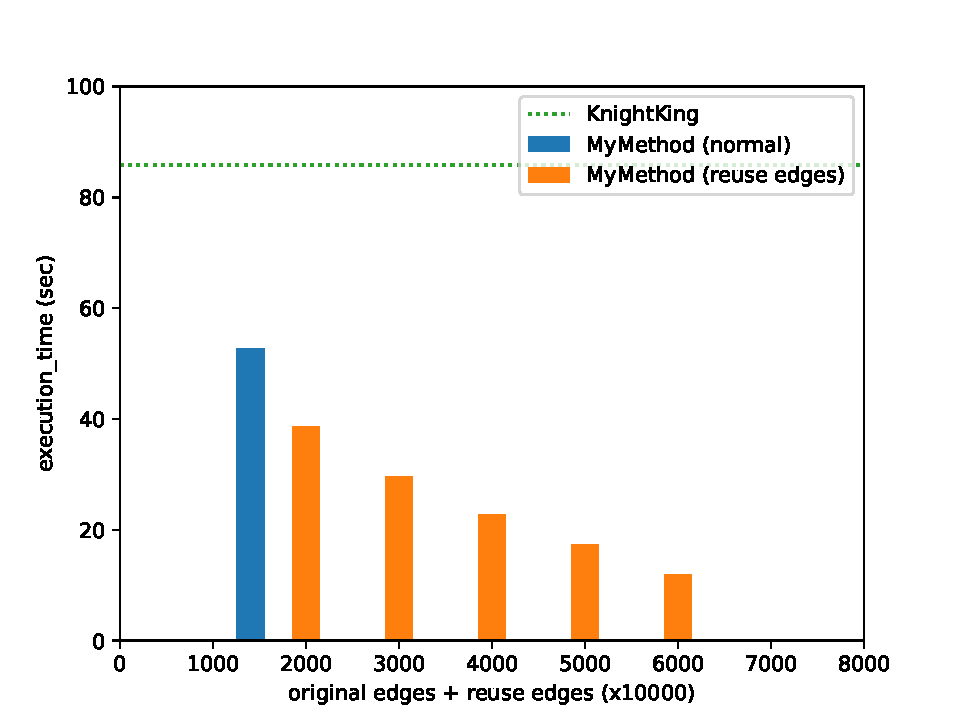
\includegraphics[scale=0.8]{figure/AR_cache.pdf}
    \caption{経路再利用をしたときの実行時間.}
    \label{経路再利用をしたときの実行時間}
\end{figure}

\subsection{グラフ分割精度を変えた場合の実行時間}\label{グラフ分割の汚さを変えた場合の実行時間}

\begin{figure}[t]
    \centering
    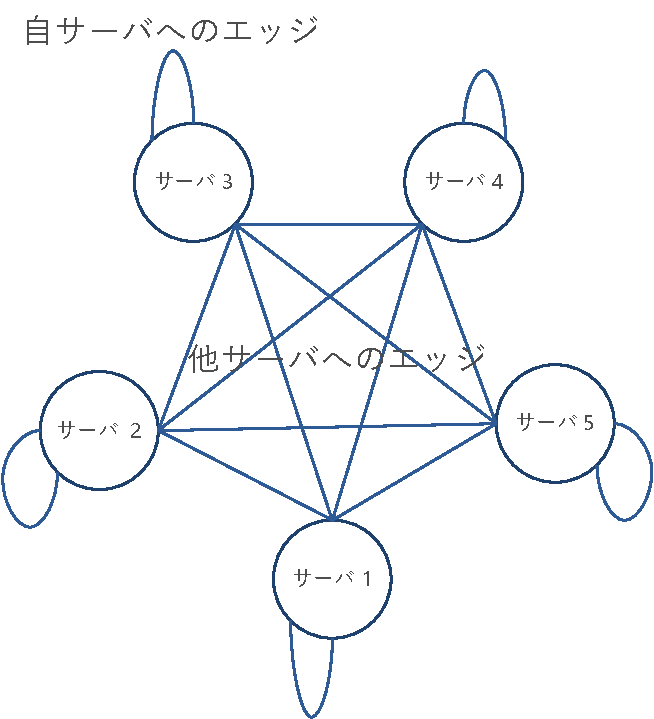
\includegraphics[scale=0.7]{figure/sbm.pdf}
    \caption{SBM による生成グラフの構造.}
    \label{SBM による生成グラフの構造}
\end{figure}

\begin{figure}[t!]
    \centering
    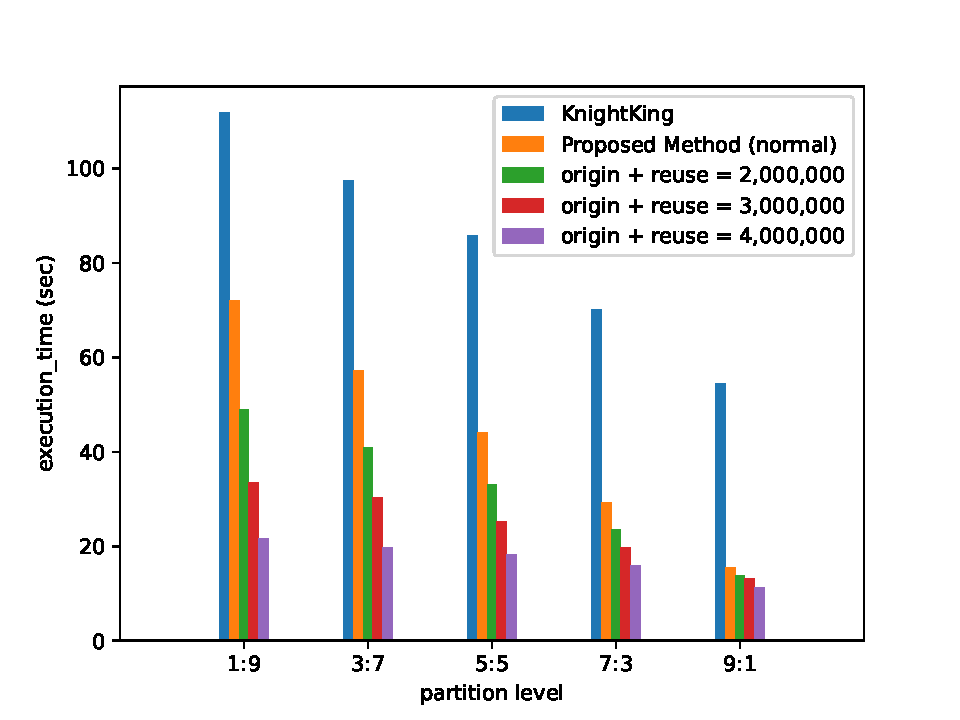
\includegraphics[scale=0.9]{figure/Kn_vs_AR_partition_level.pdf}
    \caption{グラフ分割精度を変えた場合の実行時間.}
    \label{グラフ分割の汚さを変えた場合の実行時間の結果}
\end{figure}

本実験では生成グラフを使用した. 生成グラフは SBM で作成しており, 図 \ref{SBM による生成グラフの構造} に構造を示す. SBM における partition 数 は 5, 各 partition 内の頂点数は 10000 としたため, 全グラフでの頂点数は 50000 となる. そして, partition 内の頂点間のエッジ生成確率 (自サーバへのエッジ) と partition 間の頂点間のエッジ生成確率 (他サーバへのエッジ) の比率を操作することにより, グラフ分割の精度を調節した. 例えば, 他サーバへのエッジの比率が自サーバへのエッジの比率よりも大きければ大きいほど, 他サーバが所有する頂点への RW 遷移が増えるため, サーバ間通信量が増える.  本実験においてはサーバ間通信が多くなるようなグラフ分割を精度が悪いグラフ分割であるとする. 生成確率の値については, 各サーバでのエッジ数の期待値が 1,000,000 になるように設定した. 例えば, 自サーバへのエッジ数 : 他サーバへのエッジ数 = 1 : 9 とする場合は, partition 内の頂点間のエッジ生成確率 = 0.1 \%, partition 間の頂点間のエッジ生成確率 = 0.225 \% とすることで, 自サーバへのエッジ数の期待値が 100,000, 他サーバへのエッジ数の期待値が 900,000 となり, 合計のエッジ数の期待値が 1,000,000 となる. また, サーバ数 は 5 なので, 全グラフでのエッジ数は 5,000,000 である. RW に関しては, 各頂点から 1000 回ずつ実行した. 生成グラフの頂点数は 50000 なので実行する RW 数は合計 50,000,000 回となる. また, 本実験では RWer 経路再利用機能を使用する. 

図 \ref{グラフ分割の汚さを変えた場合の実行時間の結果} にグラフ分割精度を変えたときの実行時間を示す. 横軸は自サーバへのエッジ数 : 他サーバへのエッジ数を表しており, 左に行くにつれ悪い分割になる. 横軸が 1 : 9 のとき, 提案手法は既存手法に比べてそれぞれ約 1.6 倍, 2.3 倍, 3.3 倍, 5.1 倍高速になり, 横軸が 7 : 3 のとき, 提案手法は既存手法に比べてそれぞれ約 2.4 倍, 3.0 倍, 3.5 倍, 4.4 倍高速になった. また, 提案手法における経路再利用の有無について, 横軸が 1 : 9 のとき, 経路再利用をする場合はしない場合に比べてそれぞれ約 1.47 倍, 2.15 倍, 3.32 倍高速になり, 横軸が 3 : 7 のとき, 経路再利用をする場合はしない場合に比べてそれぞれ約 1.24 倍, 1.48 倍, 1.84 倍高速になった. これらの結果から, 分割が悪ければ悪いほど, 提案手法における RWer の経路再利用の効果が大きくなるということがわかった. 地理的分散環境下では各地域ごとにグラフ編集が発生し, 全体で見たときの分割精度の制御ができないため, 分割が悪くなる場合が十分考えられるが, その場合でも提案手法は有効である. 

\subsection{グラフ分割数 (サーバ台数) を変えた場合の実行時間}\label{グラフ分割数を変えた場合の実行時間}

\begin{figure}[t]
    \centering
    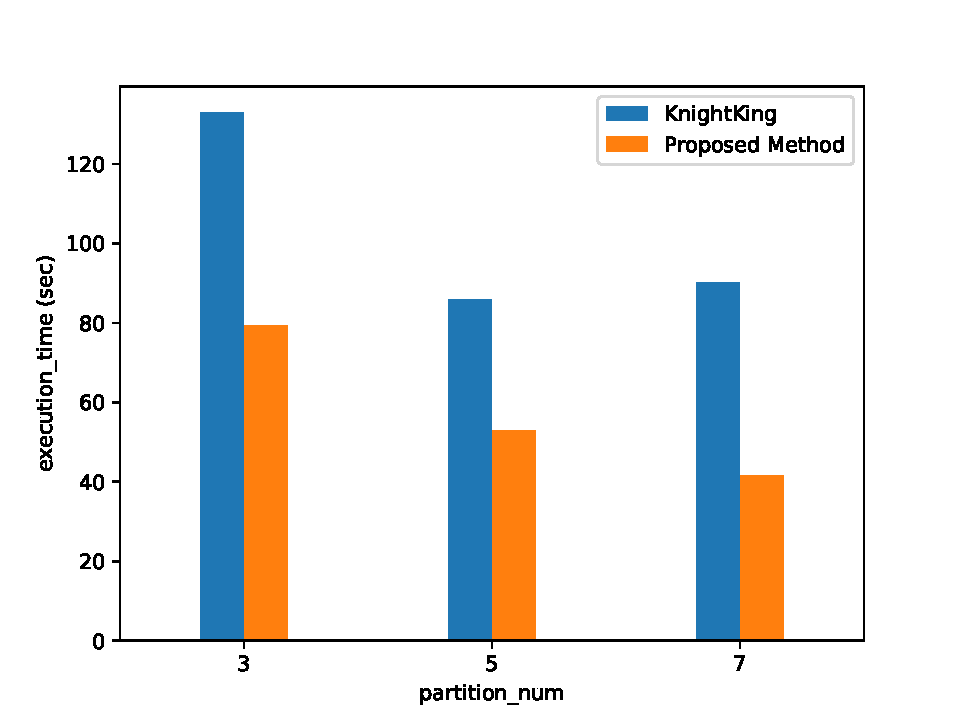
\includegraphics[scale=0.8]{figure/Kn_vs_AR_partition_num_LiveJournal.pdf}
    \caption{グラフ分割数を変えた場合の実行時間 (実世界グラフ).}
    \label{グラフ分割数を変えた場合の実行時間 (実世界グラフ)}
\end{figure}

\begin{figure}[t!]
    \centering
    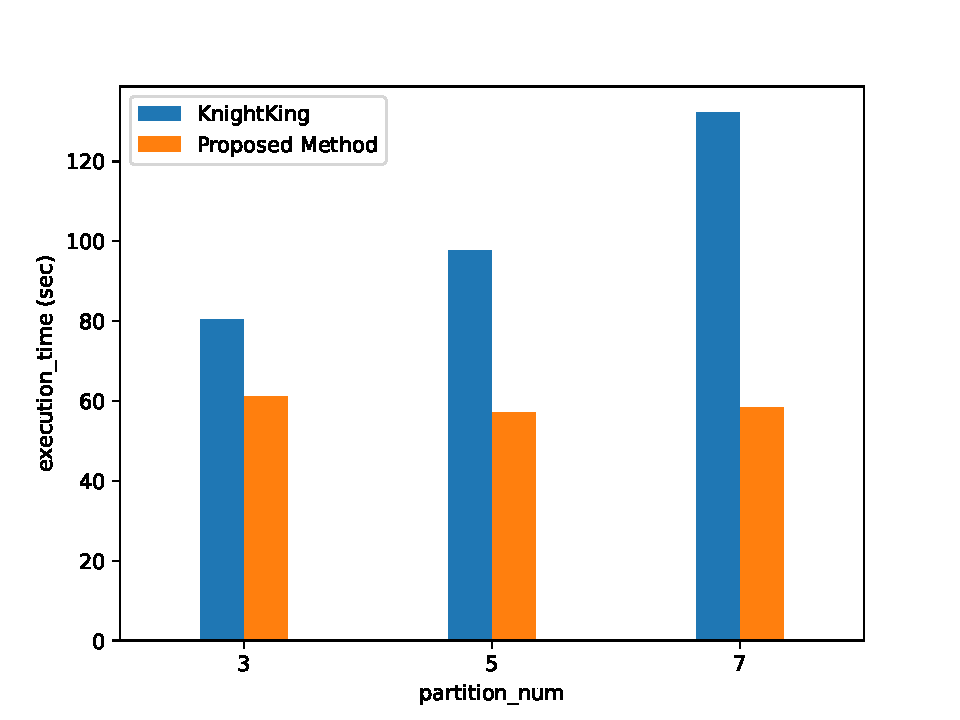
\includegraphics[scale=0.8]{figure/Kn_vs_AR_partition_num_SBM_3.pdf}
    \caption{グラフ分割数を変えた場合の実行時間 (生成グラフ).}
    \label{グラフ分割数を変えた場合の実行時間 (生成グラフ)}
\end{figure}

データセットは実世界グラフ, 生成グラフの両方を使用し, サーバ台数は 3, 5, 7 台で実験を行った. 

実世界グラフを使った実験ではサーバ台数に合わせてグラフの分割を行う. RW は各頂点から 10 回ずつ実行する. 図 \ref{グラフ分割数を変えた場合の実行時間 (実世界グラフ)} に実行時間を示す. 既存手法では, 分割数が 3 から 5 に変化した場合約 1.55 倍高速になるが, 分割数が 5 から 7 に変化した場合は約 1.05 倍遅くなる. 提案手法では, 分割数が 3 から 5 に変化した場合約 1.50 倍高速になり, 分割数が 5 から 7 に変化した場合は約 1.27 倍高速になる. この結果から分割数(サーバ台数)が 5 から 7 に変化したとき, 計算資源 (サーバ台数) の増加による高速化と通信量 (分割数) 増加による低速化に注目すると, 既存手法では通信量 (分割数) 増加による低速化が上回り, 提案手法では計算資源 (サーバ台数) の増加による高速化が上回ることがわかる. 

生成グラフを使った実験では, サーバ台数を変化させても 1 つのサーバあたりの頂点数, 辺数を変化させない (それぞれ 10000, 1,000,000) ようにグラフを生成した. つまり, サーバ台数が 3, 5, 7 と変化すると全グラフでの頂点数, 辺数は, (30000, 3,000,000), (50000, 5,000,000), (70000, 7,000,000) となる. このようにすることでシステム規模を拡大した状況を想定した実験を行うことができる. RW は各頂点から 1000 回ずつ実行する. RW 実行数の合計はサーバ台数が 3, 5, 7 と変化すると, 30,000,000, 50,000,000, 70,000,000 と変化する. 図 \ref{グラフ分割数を変えた場合の実行時間 (生成グラフ)} に実行時間を示す. 既存手法では, 分割数が 3 から 5 に変化した場合約 1.21 倍遅くなり, 分割数が 5 から 7 に変化した場合は約 1.35 倍遅くなる. 提案手法では, 分割数が 3 から 5 に変化した場合約 1.06 倍高速になり, 分割数が 5 から 7 に変化した場合は約 1.02 倍遅くなる. 実行時間に影響を及ぼすのは, 計算資源 (サーバ台数) の増加による高速化と RW 実行回数の増加と通信量増加による低速化であり, 既存手法では計算資源 (サーバ台数) の増加による高速化が上回る. 対して提案手法ではこれらがほとんど釣り合っており, 実行時間の変化が少ない. 以上の結果から提案手法は既存手法と比べシステム規模に対するスケーラビリティが高いことがわかった. 

\subsection{Random Walk の終了確率 $\alpha$ を変えた場合の実行時間}\label{終了確率 alpha を変えた場合の実行時間}

実世界グラフを用いて, 終了確率 $\alpha$ = 0.1, 0.2 の RW を各頂点から 10 回ずつ実行した. 図 \ref{alpha = 0.1 のときの実行時間} に $\alpha$ = 0.1 のときの実行時間を, 図 \ref{alpha = 0.2 のときの実行時間} に $\alpha$ = 0.2 のときの実行時間を示す. $\alpha$ = 0.1 のとき, 提案手法は既存手法に比べてそれぞれ約 1.4 倍, 1.8 倍, 2.4 倍, 3.2 倍, 4.4 倍, 6.3 倍高速になり, $\alpha$ = 0.2 のとき, 提案手法は既存手法に比べてそれぞれ約 1.9 倍, 2.6 倍, 3.3 倍, 4.1 倍, 5.0 倍, 6.5 倍高速になった. また, 提案手法における経路再利用の有無について, $\alpha$ = 0.1 のとき, 経路再利用をする場合はしない場合に比べてそれぞれ約 1.27 倍, 1.69 倍, 2.27 倍, 3.10 倍, 4.52 倍高速になり, $\alpha$ = 0.2 のとき, 経路再利用をする場合はしない場合に比べてそれぞれ約 1.35 倍, 1.73 倍, 2.14 倍, 2.62 倍, 3.42 倍高速になった. これらの結果から, 再利用エッジが増えていくと, $\alpha$ = 0.2 のときよりも $\alpha$ = 0.1 のときの方が経路再利用効果が大きくなることがわかる. これは $\alpha$ = 0.1 の方が RW の経路長の期待値が大きい(通信量が増える)ため, 経路再利用による通信スキップの恩恵が大きくなるからであると考える.
\\
\\
\\
\\
\\
\\
\\
\\
\\
\\

\begin{figure}[t]
    \centering
    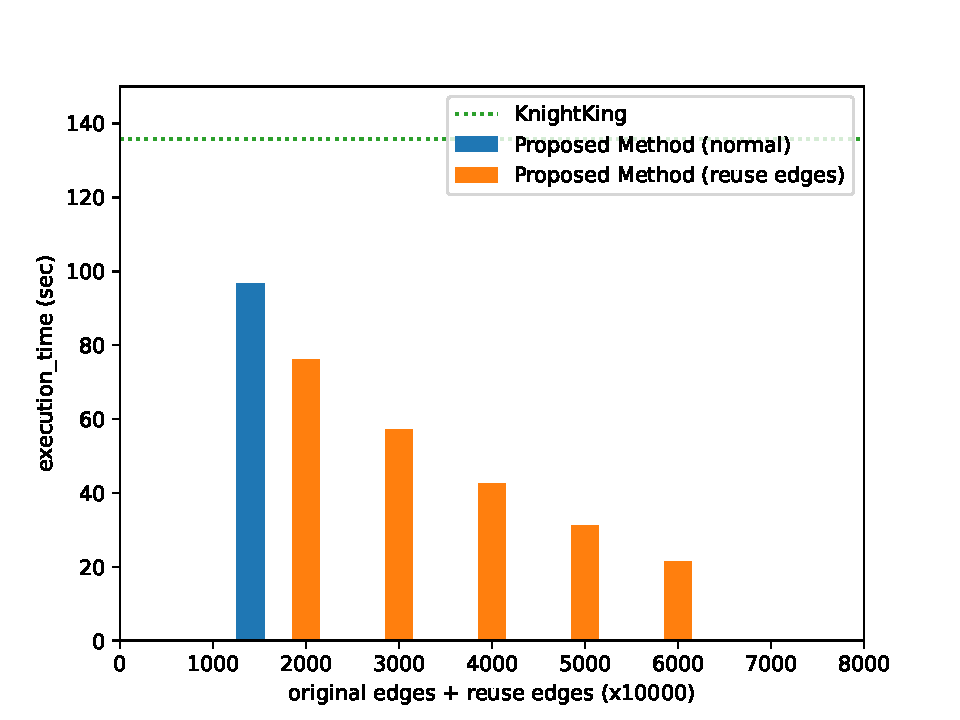
\includegraphics[scale=0.8]{figure/AR_cache_alpha_0.1.pdf}
    \caption{$\alpha$ = 0.1 のときの実行時間.}
    \label{alpha = 0.1 のときの実行時間}
\end{figure}

\begin{figure}[t!]
    \centering
    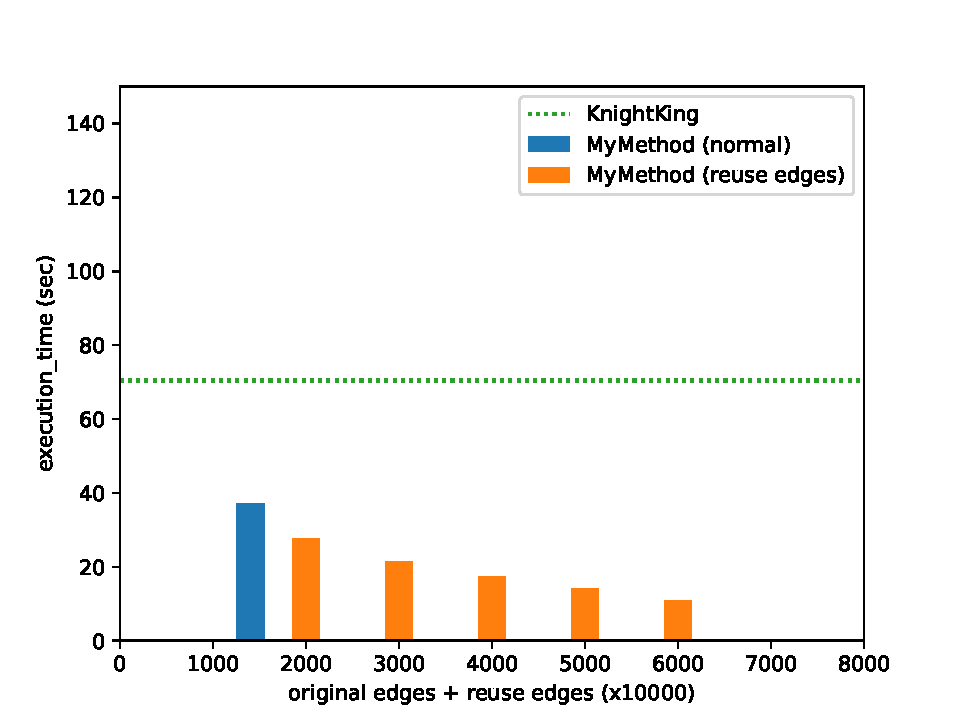
\includegraphics[scale=0.8]{figure/AR_cache_alpha_0.2.pdf}
    \caption{$\alpha$ = 0.2 のときの実行時間.}
    \label{alpha = 0.2 のときの実行時間}
\end{figure}

\section{提案手法に関する評価}

\subsection{Random Walker をまとめて送信したことによる速度向上}\label{Random Walker をまとめて送信した場合とそうでない場合の実行時間}

実世界グラフを用いて, RW を各頂点から 10 回ずつ実行した. 本実験では RWer 単体で送信する場合と複数の RWer をまとめて送信する場合の提案手法における実行時間の比較をした. 具体的には, 複数の RWer をまとめて送信する場合は \ref{sub:送信スレッド} で説明した方法で送信し, RWer 単体での送信では表 \ref{メッセージの構成} の $RWer\_count$ を必ず 1 にして送信を行う. MTU は 9000 に設定しているため, 複数の RWer をまとめる場合のパケットサイズの最大値は 9000 byte である. 
図 \ref{Random Walker の送信形態を変化させたときの実行時間} に実行時間を示す. 横軸の single が単体での送信, multi がまとめての送信を表している. 複数の RWer をまとめて送信する場合は, RWer 単体で送信するよりも 2.8 倍高速となった. 基本的にパケットサイズが大きくなればなるほどスループットが大きくなるためこの結果は妥当であり, 提案手法のように RWer をまとめて送信することが適切であるとわかった. 

\begin{figure}[t]
    \centering
    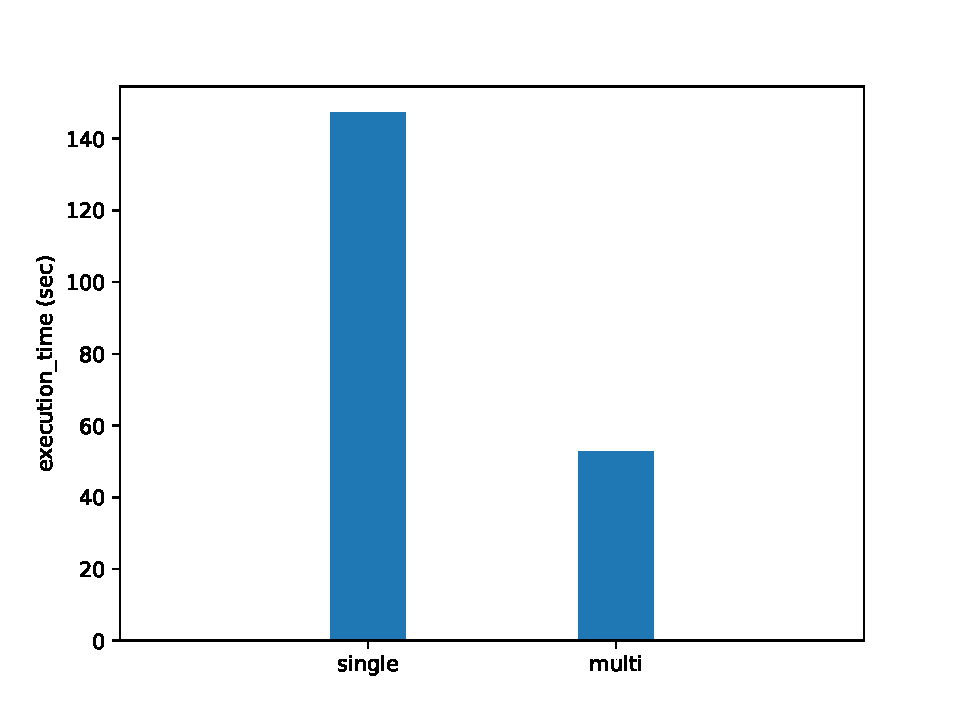
\includegraphics[scale=0.8]{figure/AR_send_num.pdf}
    \caption{Random Walker をまとめて送信したことによる速度向上.}
    \label{Random Walker の送信形態を変化させたときの実行時間}
\end{figure}

\subsection{再利用エッジが貯まるまでに実行する Random Walk の回数}\label{再利用エッジが貯まるまでに実行する Random Walk 実行数}

本実験では, 経路再利用に必要な再利用エッジが貯まるまでに必要な RW 数を測定した. 実世界グラフを用いて, RW を各サーバに規定の再利用エッジ数が貯まるまで実行し続けた. 図 \ref{再利用エッジが貯まるまでに実行する Random Walk の回数} に実験結果を示す. 横軸が各サーバに保存された再利用エッジ数, 縦軸が各サーバの RW 実行数の平均を示している. 再利用エッジ数が 6,000,000, 16,000,000, 26,000,000, 36,000,000, 46,000,000 貯まるまでに実行する RW 数はそれぞれ約 1,000,000, 3,130,000, 6,600,000, 12,000,000, 24,000,000 となった. 図 \ref{再利用エッジが貯まるまでに実行する Random Walk の回数} を見てもわかるように, 再利用エッジ数が増えれば増えるほど, さらに再利用エッジを保存するために必要になる RW 実行数が増加する. これは, RWer が同じエッジを何回も通るため新しいエッジを見つけにくくなるからである. 

\begin{figure}[t]
    \centering
    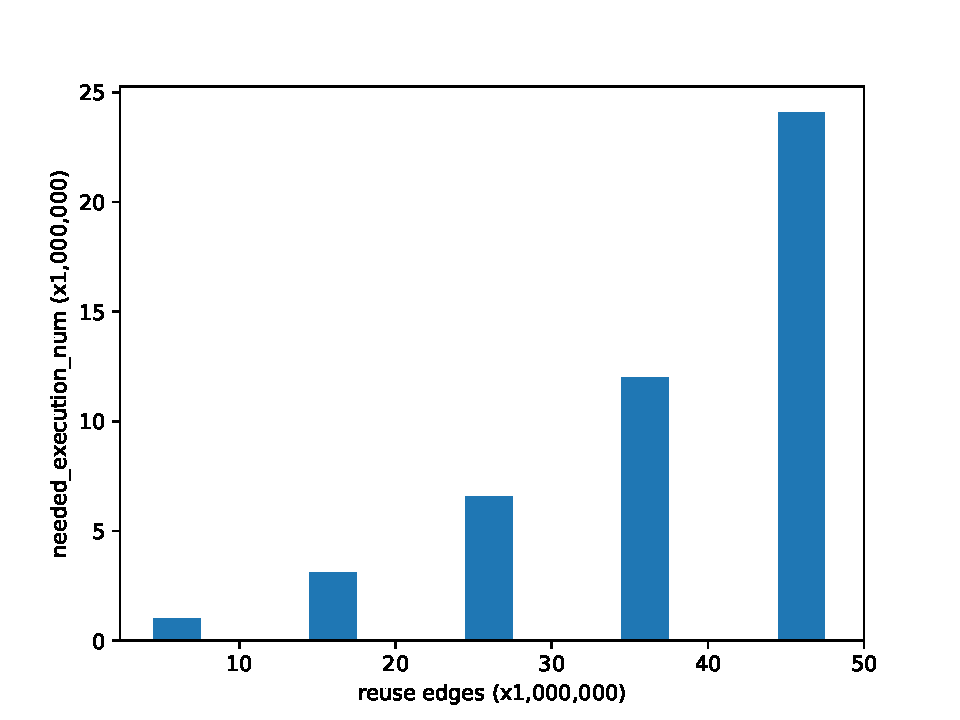
\includegraphics[scale=0.8]{figure/AR_cache_RWer_num.pdf}
    \caption{再利用エッジが貯まるまでに実行する Random Walk の回数.}
    \label{再利用エッジが貯まるまでに実行する Random Walk の回数}
\end{figure}